
\vspace*{-0.4cm}
\section{Traditional Notebooks}



We will now describe how a data scientist would perform this analysis with a traditional interactive notebook that uses Python. The description will show the issues that arise.


\eat{
\noindent {\bf Setting up and interacting  with third-party utility libraries: Productivity and security concerns.}
}


\noindent {\bf Interacting  with third-party utility libraries: Productivity and security concerns.}


\eat{ Before even starting working on any of the afore-mentioned tasks the data analyst must make sure that all third-party python packages that will be used for retrieving and visualizing data, are installed. This step will either introduce a dependency between the analyst and some system administrator, or the analyst will need the appropriate access rights in order to perform the installation, typically, using a command line. The latter can be a security concern (especially, if the server on which the notebook operates, also hosts other applications) and can also lead to corrupted systems if not performed correctly. The complexity of this step increases as the number of utility libraries, our analyst wants to use, increases. \eat{More specifically, for cases when an analyst needs to access data stored in a MongoDB and a MySQL database, two drivers will need to be installed.}
}
\begin{figure*}[hbt!]
\centering
	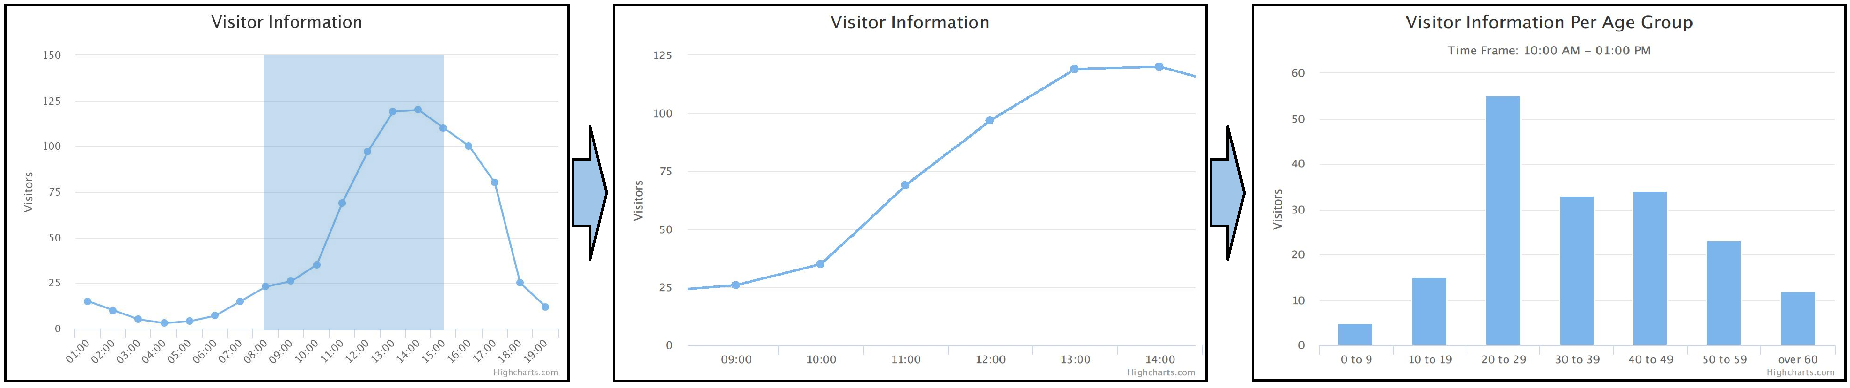
\includegraphics[width=1\textwidth]{figures/reactive-processing2.pdf}
	\caption{Demonstration of reactive charts. The reader's selection automatically updates both charts.}
	\label{fig:reactive-data-processing}
	\vspace{-10pt}
\end{figure*}


In order to retrieve website access information from the database, the data analyst, needs to employ third-party Python drivers. Employing such drivers, involves reading lengthy documentation pages that describe the exposed API calls of the respective driver. After identifying the appropriate API calls, the analyst needs to use imperative logic that interacts with the library, in order to issue the appropriate query. During this step, the analyst has to also specify the credentials that will be used for accessing the database system. In most such libraries, the credentials have to be inlined into the method call that establishes the connection with that system. While this would not be a security concern in a python (or any other) application (since the code that includes the credentials would have been compiled into a binary file, thus hiding them), in a python notebook, the credentials would lie in plain sight for anyone, who has access to the notebook, to see. This security concern is also resolved in \projname. \costas{Is the security aspect of it a weak point? Should I remove it?}

\costas{reviewer 1: c. Logging into databases, etc using Python libraries is not really harder today than what you show in the paper. See the ipython-sql library and its use of SQLAlchemy. For us database folks, this is already a standard way to work with Python and notebooks. d. You seem to indicate that there is an unsolved object-relational data type conversion problem in Python/SQL. But Pandas dataframes do a fine job with this, even over something like ipython-sql. This is a non-issue for Python notebook users today. }

\costas{ipython-sql is a python magic command that let's you inline queries in Jupyter and it returns the result in a pandas dataframe. This tool lacks the interactive aspect which is required in order to build a reactive analysis. You cannot issue a parameterized query that is executed every time the user interacts with a visualization (I verified this).}

\noindent {\bf Data conversions.} 
After, establishing the connection with the database system, and issuing the queries, the analyst, is able to consume the results by using the internal, to the library, data types. After doing so, the analyst has to again read documentation pages in order to infer the data types required by the visualization library she selected, and manually perform the appropriate conversions in order to construct the first visualization, by invoking the appropriate renderer function. Note that data conversions have to take place every time the analyst wishes to integrate a third-party library in her analysis, so the amount of plumbing code required, can quickly skyrocket.


\costas{Repeating comment here: d. You seem to indicate that there is an unsolved object-relational data type conversion problem in Python/SQL. But Pandas dataframes do a fine job with this, even over something like ipython-sql. This is a non-issue for Python notebook users today. Separate comment: It felt to me that you are unfamiliar with Jupyter Lab, Pandas, and the rest of the standard toolchain that people use. Maybe that's not true! But it comes across that way. For example, it's odd that you return dictionaries rather than dataframes, and your comments on "Data conversion" reinforces that feeling. If you do know your stuff, then for some reason you are not integrating with the community's favorite libraries. If that's the case, you might be more thoughtful in explaining why your counter-cultural approach is good.}

\costas{The point I was trying to make here is that regardless of whether we integrate with dictionaries or dataframes, the analyst still has to read the documentation page of the visualization library and manually convert the data into the format/schema that is expected by the visualization library. Dataframes are indeed used a lot by many libraries however they cannot capture nested data while dictionaries can. Additionally, dictionaries are natively supported by Python while Pandas is an external library. Also while some tools interface well with pandas many of them actually require conversions into python dictionaries/arrays (here is an example using plotly that requires a dataframe to be converted into a dictionary: https://plot.ly/ipython-notebooks/cufflinks/, plotly has the same issue) as shown in the same link because of this missmatch, additional libraries have to be used to simplify this data conversion (i.e., cufflinks). On the other hand all libraries interface with python natively supported types (i.e., dictionaries) additionally dataframes can be converted into (flat) dictionaries with one command (and the other way around)... If he considers integration with dataframes (which again are simply flat dictionaries) so critical, we can support that as well. On a separate note, Jupyter Labs is simply a more advanced web IDE for creating ipython notebooks. I don't understand how that's comparable to vidette (one can use Jupyter labs to build a jupyter notebook that employs vidette...)}

\noindent {\bf Limited interactive exploratory capabilities.}
The next step, is for the analyst to issue a query that counts the visitors per age group for a set of selected hours and construct a bar chart showing the result. The obtained dataset will also go through a machine learning package (for instance, the scikit-learn package \cite{scikit-learn}), that employs a linear regression model to predict the expected revenue during the selected hours. The predicted revenue will be plotted next to the actual revenue produced during these hours. Note that selecting a meaningful time frame, is of utmost importance, because it will affect all the remaining steps of this analysis, and ultimately the insight, the portal editor will gain, about potential ways to increase the revenue. 




 % Template and template instance figures
 \begin{figure*}[hbt!]
 \centering
 %
 %
 \begin{minipage}[c]{7cm}
 %
 \begin{minipage}[c]{7cm}
 \begin{code}
 \textbf{<\% let} readings = 
    SELECT count(time) as visits, time
    FROM (SELECT * FROM page_views pv 
   	     join visitors v 
          on pv.v_id = v.vid) AS joined_table
    GROUP BY time 
    ORDER BY time ASC \textbf{\%>};
 \end{code}
 \vspace*{-0.4cm}
 \subcaption{Data retrieval}
 \label{figure:first-running-example:data-retrieval}
 \vspace*{0.3cm}
 \end{minipage}
 \begin{minipage}[c]{7cm}
 \begin{code}
 readings = [
    \{visits: 15, time: '08:00'\}, 
    \{visits: 10, time: '09:00'\},
    \{visits: 25, time: '10:00'\},  ...]
 \end{code}
 \vspace*{-0.4cm}
 \subcaption{Query Result}
 \label{figure:running-example:query-result}
 \vspace*{0.3cm}
 \end{minipage}
 \begin{minipage}[c]{7cm}
 \begin{code}
 sources : [ \{ 
      driver   : "postgres", 
      host     : "edu.db.domain", 
      expose   : [ \{
       schema : 'website_info', 
       tables: [visits, page_views] \} ]
      port     : 5432, 
      username : "dbadmin" 
      password : 'myP@ss'
    \}] 
 \end{code}
 \vspace*{-0.4cm}
 \subcaption{DB Access Configuration file}
 \vspace*{0.3cm}
 \label{figure:source-config-file}
 \end{minipage}
 %
 \vspace*{0.6cm}
 \end{minipage}
 \hspace{2cm}
 \begin{minipage}[c]{6cm}
 \begin{minipage}[c]{7.5cm}
 \begin{code}
   \directive{unit}{highcharts} \{
     title: 'Visitor information' ,
     type: 'line',
     xAxis : \{ 
       labels : ['08:00','09:00'...],
       min : '08:00'
       max : '22:00'
     \}
     series: [\{ data: [ \{y:15\}, \{y:10\}...] \}]
   \} \directive{end unit}{}
 \end{code}
 \vspace*{-0.4cm}
 \subcaption{Unit with evaluated unit state}
 \vspace*{0.3cm}
 \label{figure:running-example:unit-body}
 \end{minipage}
 \begin{minipage}[c]{7.5cm}
 \begin{code}
   \directive{unit}{highcharts} \{
     title: 'Visitor information',
     type: 'line',
     xAxis : \{ 
       labels : [
         \directive{for}{reading \textbf{in} readings} 
           \directive{print}{reading.time} 
         \directive{end for}{}],
       min : \directive{bind}{min_time},
       max : \directive{bind}{max_time}
     \}
     series: [\{
       data: [ \directive{for}{reading \textbf{in} readings}
           \{
             y  : \directive{print}{reading.count}
           \}
         \directive{end for}{} ]
     \}]
   \} \directive{end unit}{}
 \end{code}
 \vspace*{-0.3cm}
 \subcaption{Template generating unit state of first chart}
 \vspace*{0cm}
 \label{figure:first-running-example:main-template}
 \end{minipage}
 \end{minipage}
 \vspace*{-0.3cm}
 \caption{Declarative Data retrieval, DB Configuration, evaluated unit state and Template describing unit state for running example}
 \vspace*{-0.3cm}
 \end{figure*}
 Unfortunately, there is no straightforward way for selecting a meaningful time frame. The analyst will have to go through a process of trial and error, by issuing an arbitrary number of such queries and plotting the results, until she finds a set that produces valuable insight. Furthermore, even if the analyst goes through this process for the data corresponding to a particular day, the time frame selection she made, might not produce any valuable insight for the dataset corresponding to another day. Most importantly the non-technical reader cannot use the notebook to test similar hypotheses, she is limited to passively reading the ones that were hardcoded by the analyst. This aspect of introducing the human in the loop is improved dramatically with \projname\ notebooks.
 

